
\section{Our Colossal Approach}
\label{sec:sec3}

As we illustrated in Section \ref{sec:sec2}, the cluster operations
team has to answer a large number of questions in order to manage
multi-tenancy. Broadly, we can categorize these questions into
three categories. 

\squishlist

\item {\em What-is questions:} These are questions aimed at gaining
a deeper understanding of multi-tenancy in the cluster. Examples 
that we saw in Section \ref{sec:sec2} include 
understanding the effective utilization of the overall cluster 
as well as the effective utilization of different pools. 

\item {\em What-if questions:} These are questions aimed 
at understanding the impact of various changes. Examples include
understanding the impact of: (a) an increase in a pool's 
workload, (b) a change in a pool-level configuration
parameter such as the preemption timeout, 
and (c) a change in the layout of a table.

\item {\em What-should questions:}  These are questions aimed 
at identifying the best configurations for tunable parameters
given constraints and/or an optimization objective. 
An example is to find the best setting of pool-level 
configuration parameters for all pools in order to satisfy 
constraints (SLAs) on average completion time in some pools, 
while maximizing the overall cluster utilization. 

\squishend

{\em Colossal} is a platform that we are developing to 
enable cluster operators to get answers to such questions 
easily. In this section, we will describe the five main
components of Colossal and our current implementation of each component. 
Each component is designed to be pluggable and can have different 
implementations.

\subsection{Extractors}
An {\em Extractor}'s goal is to generate a workload model
from raw traces of workload execution. The main reason
for generating workload models is to enable anwering
What-if questions of the form: what is the impact of  
a 5\% increase in the workload of the BI pool? 
Workload models enable concrete descriptions of 
what a 5\% increase in a particular workload means.  

We have implemented an Extractor for the workload 
seen on Rocket Fuel's multi-tenant cluster. This Extractor
takes as input all job history logs generated
by Hadoop for some period of time. From a statistical analysis
of the workload, we observed that the job
arrival follows a Poisson process with a relatively constant
arrival rate for each pool. In addition, the map and reduce attempt
duration follows a lognormal distribution (which is similar
to the observations in \cite{taobao-paper}). 
The task count of a job can also be approximated using a lognormal
distribution for each pool. Thus, the Extractor uses 
maximum likelihood estimation of parameters to fit 
the observed distributions. Table \ref{tab:workload-model}
shows the best-fit workload model for the BI pool.

\begin{table*}
  \centering
  \caption{Workload model of analyst pool (Time is in seconds)}
  \begin{tabular}{|c|c|l|} \hline
    Parameter&Description&Estimated Value\\ \hline
    job\_arrival\_rate & Number of job arrivals per second &
    0.00282392166\\ \hline
    logmean\_maps\_per\_job & Mean of the logarithm of job map count & 4.860108\\ \hline
    logmean\_reduces\_per\_job & Mean of the logarithm of job reduce count & 1.720507\\ \hline
    logsd\_maps\_per\_job & Standard deviation of the logarithm of job map count & 3.202215\\ \hline
    logsd\_reduces\_per\_job & Standard deviation of the logarithm of job reduce count & 2.540193\\ \hline
    logmean\_map\_duration & Mean of the logarithm of job task duration & 3.765196\\ \hline
    logmean\_reduce\_duration & Mean of the logarithm of reduce task duration & 5.154496\\ \hline
    logsd\_map\_duration & Standard deviation of the logarithm of map task duration & 0.8837955\\ \hline
    logsd\_reduce\_duration & Standard deviation of the logarithm of reduce task duration & 2.043326\\ \hline
\end{tabular}
\label{tab:workload-model}
\end{table*}

\subsection{Transformers}
A {\em Transformer}'s goal is to generate an actual 
specification of a workload that will be input  
to the {\em Predictor}. We have implemented two different
Transformers so far. A simple Transformer takes the 
raw Hadoop job history logs and transforms it to the 
workload input specification supported by the Predictor. 
The more complex Transformer that we have implemented 
can take the workload model learned by the Extractor 
from the previous section, and generate various scaled versions
of the workload along different dimensions. For example, 
this Transformer can generate a workload 
with a 5\% increase in the number of map tasks per job
in order to represent a 5\% increase in overall
data volume. 

In future, we will be supporting more sophisticated
Transformers to connect Colossal with other tuning tools
in order to answer questions of the form: What will be the overall 
impact of changing the data layout of a table $T$? 
To answer this question, a data-layout tuning tool (external
to Colossal) will have to provide Colossal's Predictor with 
the new workload that will result from 
changing the data layout of table $T$. In this way, Colossal
will be able to apply a divide-and-conquer approach to 
answer hard questions in multi-tenancy that cluster operators 
have no way of answering today. 

\subsection{Predictors}
A {\em Predictor} takes three inputs: (i) a multi-tenant workload, 
(ii) pools and their configuration, and (iii) 
cluster resource configuration. The goal of the Predictor
is to output the predicted schedule of execution
of the workload on the cluster. In addition, the Predictor
also outputs standard performance metrics associated with 
a multi-tenant workload. 

The Predictor has to be both fairly accurate as well as 
highly efficient in performance prediction. As we will 
see in Section \ref{sec:optimizer}, {\em Optimizers} may have 
to call the Predictor multiple times. We could not 
use a number of Hadoop simulators that have 
been developed in the past either because they 
were inefficient in handling large workloads or 
were too inaccurate due to assumptions made 
regarding multi-tenancy \cite{sls,mr-sim}. 

Our current implementation of the Predictor is for a 
cluster where the multi-tenancy is enforced by the Hadoop
Fair scheduler. This Predictor is based on a novel algorithm
which simulates the Fair scheduler in accelerated {\em virtual
time}. Given the workload trace for an interval $T$, the predictive
algorithm will require a much shorter run-time $t$ << $T$ to produce the
predicted results. For example, the Predictor requires less than 
4 minutes (a significant fraction of which is I/O time for 
the large workload file) to generate 
performance predictions for one week of Rocket Fuel's workload.

The key idea used in the predictive algorithm is to map events---such as
preemptions, job starts, and job completions---on to a virtual timeline. A
finite state machine is then established to process the events in the
increasing order of virtual time. While processing an event, the state
machine may also alter later events in the virtual timeline, but
not the earlier ones. Thus, the running time of the algorithm is
proportional to the number of tasks, jobs, and preemptions.
This approach has
the advantage over most previous approaches in which the running time of
simulation also depends on the running time of jobs
\cite{sls,conf/cluster/VermaCC11,mr-sim}.

\subsection{Inspectors}

Once the Predictor or Optimizer 
has generated its output, an {\em Inspector}'s
role is to help the operations team get the answer to 
their question from the output. In many cases, the 
overall understanding of the operations team can be further improved by 
visualizing the time series of metrics in the output. 
Our current implementation of Inspectors 
provides visualizations for several built-in performance metrics 
such as effective utilization as
described in the previous section, average job latency for
each pool, and others. 

\begin{figure}
  \centering 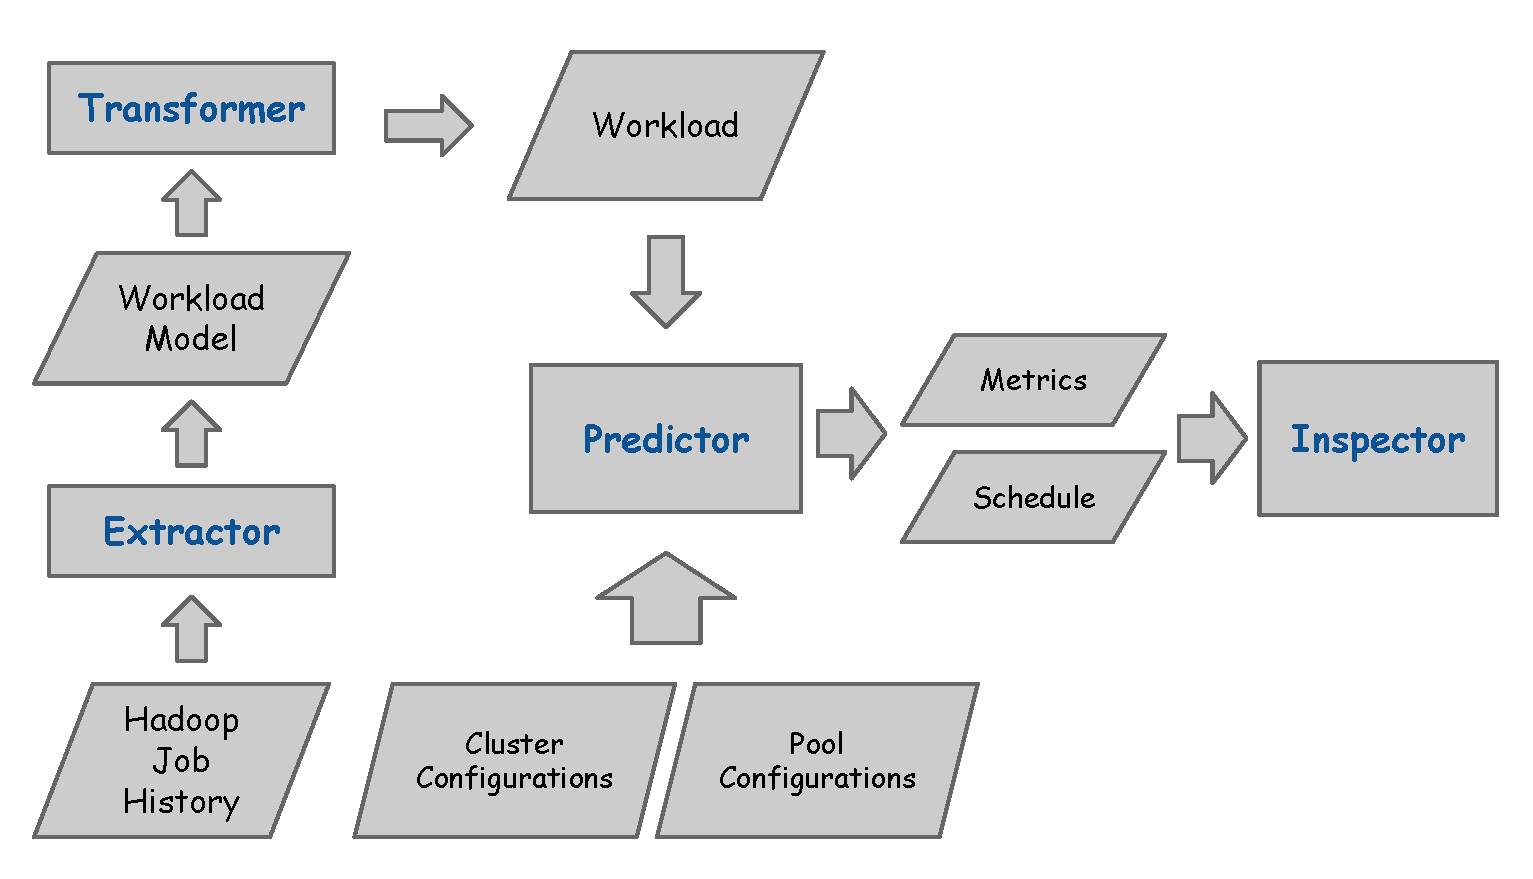
\epsfig{file=arch.eps,scale=0.3}
  \caption{Overview of the Colossal Platform}
  \vspace{-6mm}
\end{figure}

\subsection{Optimizers}
\label{sec:optimizer}

The role of an {\em Optimizer} in the 
Colossal platform is to find configuration parameter settings that 
optimize user-specified performance metrics
in a multi-tenant cluster. The optimization is done by 
searching over the possible parameter space, and 
calling into the Predictor in order to estimate performance
for selected configuration parameter settings. The search process 
is made efficient by parallelizing using MapReduce as well as 
using heuristics to prune the search space dynamically.

Specifically, a user can define an objective function {\em F(M,S)} 
where $M$ and $S$ are, respectively, the output metrics and
schedule from the Predictor. Typical objective functions use
three of the built-in metrics:
(a) {\em AvgJobLatency}, which represents the average job
latency of each pool, (b) {\em Throughput}, which represents the throughput
(number of jobs per second) of each pool, and (c) {\em EffectiveUtil}, 
which represents the effective utilization defined in 
Section \ref{sec:sec2}. Additionally,  users 
specify the parameters (i.e., the free variables in the search) 
for which they want recommended settings. For example, 
any subset of the configuration parameters listed in 
Table \ref{tab:scheduler-config} can be specified 
as free variables. 

